\section{Heapsort}

\subsection{Heaps}

\begin{description}
  \item[6.1-1] {\itshape What are the minimum and maximum numbers of elements in a heap of height $h$?} %TODO:TikZ heap diagram
    \begin{ex}
      \begin{itemize}
        \item Minimum : $2^{h}$ ;
        \item Maximum : $2^{h+1}-1$ .
      \end{itemize}
    \end{ex}
  \item[6.1-2] {\itshape Show that an $n$-element heap has height $\lfloor \lg n \rfloor$.}
    \begin{ex}
      On reprend le r\'esultat pr\'ec\'edent qui nous offre une in\'egalit\'e :
      $$2^h \le n \le 2^{h+1}-1.$$
      Ainsi, \'etant donn\'e un nombre d'\'el\'ements $n$, l'hauteur $h$ d'un tas est born\'ee par :
      $$\lg n -1  < \lg(n+1)-1 \le h \le \lg n.$$
      Sachant que $h$ est un entier, de $\lg n - 1 < h \le \lg n$ on d\'eduit que $h = \lg n$.
    \end{ex}
  \item[6.1-3] {\itshape Show that in any subtree of a max-heap, the root of the subtree contains the largest value occurring anywhere in that subtree.}
    \begin{ex} %TODO:give a complet proove
      C'est une cons\'equence imm\'ediate de la propri\'et\'e d'un {\itshape max-heap} : la cl\'e de la racine d'un sous-arbre est sup\'erieur \'egale \`a celle de ses enfants; or, ses enfants sont \'egalement la racine du sous-arbre qu'ils apartiennent. De ce fait, une preuve plus compl\`ete serait achev\'ee par induction math\'ematiques.
    \end{ex}
  \item[6.1-4] {\itshape Where in a max-heap might the smallest element reside, assuming that all elements are distinct?}
    \begin{ex}
      La propri\'et\'e d'un {\itshape max-heap} est que $A[\proc{Parent}(i)] \ge A[i]$ ce qui signifit que tout chemin partant de la racine forme une suite d\'ecroissante, et strictement, par hypoth\`ese. Par cons\'equence, le plus petit \'el\'ement r\'eside dans une des feuilles. Ce r\'esultat d\'ecoule du fait que la relation d'ordre n'est pas totale sur le tas.
    \end{ex}
  \item[6.1-5] {\itshape Is an array that is in sorted order a min-heap?}
    \begin{ex}\mbox{}\\ %TODO:add proof
      Si le tableau est tri\'e de mani\`ere croissante, le tableau forme un {\itshape min-heap}.
    \end{ex}
  \item[6.1-6] {\itshape Is the array with values $\langle 23, 17, 14, 6, 13, 10, 1, 5, 7, 12\rangle$ a max-heap?}
    \begin{ex}
      Consid\'erons la figure (\ref{fig:6.1-6}) qui est la repr\'esentation arborescente du tableau. On voit qu'il existe une sous suite qui n'est pas d\'ecroissante : $\langle 23, 17, 6, 7\rangle$, donc ce tableau ne v\'erifie pas la propri\'et\'e d'un \textit{max-heap}.
        \begin{figure}[H]
          \centering
        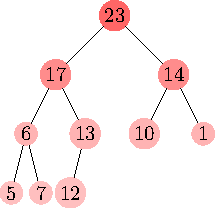
\includegraphics[scale=1.5]{img/6_1-6/6_1-6.pdf}
        \caption{Tas sous forme d'arbre du tableau $\langle 23, 17, 14, 6, 13, 10, 1, 5, 7, 12\rangle$}
          \label{fig:6.1-6}
        \end{figure}
    \end{ex}
  \item[6.1-7] {\itshape Show that, with the array representation for storing an $n$-element heap, the leaves are the nodes indexed by $\lfloor n/2 \rfloor +1, \lfloor n/2\rfloor + 2, \ldots, n$.}
    \begin{exrev}
      
    \end{exrev}
\end{description}
